\documentclass[12pt]{article}

% -----------------------------
% Packages
% -----------------------------
\usepackage[utf8]{inputenc}
\usepackage[T1]{fontenc}
\usepackage{lmodern}
\usepackage[most]{tcolorbox}
\usepackage{amsmath, amssymb, amsthm}
\usepackage{mathtools}
\usepackage{physics}          % Derivatives, vector notation, etc.
\usepackage{bm}               % Bold math symbols
\usepackage{cancel}           % For striking out terms
\usepackage{xcolor}           % For highlighting
\usepackage[dvipsnames]{xcolor}
\usepackage{tikz}             % Diagrams
\usepackage{tikz-3dplot}
\tdplotsetmaincoords{70}{110}
\usepackage{enumitem}         % Customizable lists
\usepackage{hyperref}         % Clickable references
\usepackage{geometry}         % Page margins

% -----------------------------
% Geometry
% -----------------------------
\geometry{margin=1in}

% -----------------------------
% Theorem / Definition Styles
% -----------------------------
\newtheorem{theorem}{Theorem}[section]
\newtheorem{lemma}[theorem]{Lemma}
\newtheorem{proposition}[theorem]{Proposition}
\newtheorem{corollary}[theorem]{Corollary}
\newtheorem{definition}[theorem]{Definition}
\newtheorem{example}[theorem]{Example}
\newtheorem{remark}[theorem]{Remark}

% -----------------------------
% Common Sets
% -----------------------------
\newcommand{\R}{\mathbb{R}}
\newcommand{\N}{\mathbb{N}}
\newcommand{\Z}{\mathbb{Z}}
\newcommand{\Q}{\mathbb{Q}}
\newcommand{\C}{\mathbb{C}}

% -----------------------------
% Linear Algebra Shortcuts
% -----------------------------
\newcommand{\vect}[1]{\mathbf{#1}}          % Vectors in bold
\newcommand{\mat}[1]{\mathbf{#1}}           % Matrices in bold
\newcommand{\inv}{^{-1}}                    % Inverse
\DeclareMathOperator{\Span}{span}
\DeclareMathOperator{\nullity}{nullity}
\DeclareMathOperator{\diag}{diag}
\DeclareMathOperator{\Det}{det}

% -----------------------------
% Differential Equations Shortcuts
% -----------------------------
\newcommand{\ddx}{\frac{d}{dx}}
\newcommand{\ddy}[1]{\frac{d}{d#1}}
\newcommand{\ppx}{\frac{\partial}{\partial x}}
\newcommand{\ppy}[1]{\frac{\partial}{\partial #1}}

% Dot notation for ODEs
\newcommand{\dotx}{\dot{x}}
\newcommand{\doty}{\dot{y}}
\newcommand{\dotz}{\dot{z}}

% -----------------------------
% Hyperref Setup
% -----------------------------
\hypersetup{
    colorlinks = true,
    linkcolor  = blue,
    urlcolor   = teal,
    citecolor  = magenta
}

% -----------------------------
% Stylistic Options and Aux Settings
% -----------------------------

\setlength{\parindent}{0pt}
\allowdisplaybreaks
\tcbset{problem/.style={colback=Gray!20, colframe=Black, breakable, enhanced jigsaw, arc=0.5mm, boxrule=0.5pt}}


% -----------------------------
% Document Info
% -----------------------------
\title{Linear Algebra and Differential Equations}
\author{Lecture Notes}
\date{August 27, 2025}

\begin{document}

\maketitle      % Inputting Document Info

At the core, linear algebra surrounds the solving of systems of equations. Take the following linear system for instance: \par
\begin{tcolorbox}[problem]
    \vspace{-12pt}
    \begin{align*}
        2x_1 + 3x_2 &= 10 \\
        4x_1 + 11x_2 &= 16
    \end{align*}
\end{tcolorbox}

Traditionally, one of two methods is employed. One can use elimination to eliminate a variable: \par
\begin{tcolorbox}[problem]
    We first begin by multiplying the first equation by $-2$.
    \begin{align*}
        -2(2x_1 + 3x_2) &= -2(10) \\
        4x_1 + 11x_2 &= 16 \\[12pt]
        -4x_1 + -6x_2 &= -20 \\
        4x_1 + 11x_2 &= 16
    \end{align*}
    We then sum both equations to eliminate $x_1$. \begin{align*}
        -4x_1 + -6x_2 + (4x_1 + 11x_2) &= -20 + 16 
    \end{align*}
    This leaves us with: \begin{align*}
        5x_2 &= -4 \\[6pt]
        x_2 &= -\dfrac{4}{5}
    \end{align*}
    We can then substitute $x_2$ back into equation $1$ to find $x_1$. \begin{align*}
        2x_1 + 3\left(-\dfrac{4}{5}\right) &= 10 \\[6pt]
        2x_1 - \dfrac{12}{5} & = 10 \\[6pt]
        2x_1 &= \dfrac{62}{5} \\[6pt]
        x_1 &= \dfrac{31}{5}
    \end{align*}
    Therefore, our solution set is: \begin{align*}
        \boxed{(x_1, x_2) = \left(\dfrac{31}{5}, -\dfrac{4}{5}\right)}
    \end{align*}
\end{tcolorbox}

The other method traditional method for solving linear systems is solving one variable in terms of another: \par
\begin{tcolorbox}[problem]
    We can first express $x_1$ in terms of $x_2$. \begin{align*}
        x_1 = \dfrac{10 - 3x_2}{2}
    \end{align*}
    We can then substitute $x_2$ for $x_1$ in the second equation. \begin{align*}
        4\left(\dfrac{10 - 3x_2}{2}\right) + 11x_2 = 16
    \end{align*}
    Now, we are able to solve for $x_2$. \begin{align*}
        \dfrac{40 - 12x_2}{2} + 11x_2 &= 16 \\[6pt]
        \dfrac{40 - 12x_2 + 22x_2}{2} & = 16 \\[6pt]
        40 + 10x_2 &= 32 \\[6pt]
        10x_2 &= -8 \\[6pt]
        x_2 &= -\dfrac{4}{5}
    \end{align*}
    Again, as shown above, we can now substitute $x_2$ back into equation $1$ to find $x_1$. Our solution once again turns out to be \begin{align*}
        \boxed{(x_1, x_2) = \left(\dfrac{31}{5}, -\dfrac{4}{5}\right)}.
    \end{align*}
\end{tcolorbox}

However, what if we have 10 equations and 10 variables? It's clear that although we could use the aforementioned methods, there would be many more steps and will take much longer. This is where linear algebra comes in. There are primarily two contexts where linear algebra is especially useful. \par

\newpage

\textbf{Context 1: Extension into Multiple Dimensions} \par

Imagine you have a 3D space, and in that 3D space, there lies a plane and a point. \par

\begin{center}
    \begin{tikzpicture}[tdplot_main_coords, scale=3]

        % axes
        \draw[->] (0,0,0) -- (1.2,0,0) node[below] {$x$};
        \draw[->] (0,0,0) -- (0,1.2,0) node[right] {$y$};
        \draw[->] (0,0,0) -- (0,0,1.2) node[above] {$z$};
      
        % define a "plane" as a quadrilateral
        \filldraw[fill=blue!20, opacity=0.5]
          (0,0,0.5) -- (1,0,0.5) -- (1,1,0.5) -- (0,1,0.5) -- cycle;
        \node at (0.5,0.5,0.55) {};
      
        % point in space
        \filldraw[red] (0.5,0.5,1) circle (0.5pt) node[above right] {$P$};
      
      \end{tikzpicture}
\end{center}

To find the distance from point $P$ to the plane, one can use many methods, including but not limited to using the distance formula or using the cross product. \par

\begin{center}
    \begin{tikzpicture}[tdplot_main_coords, scale=3]

        % axes
        \draw[->] (0,0,0) -- (1.2,0,0) node[below] {$x$};
        \draw[->] (0,0,0) -- (0,1.2,0) node[right] {$y$};
        \draw[->] (0,0,0) -- (0,0,1.2) node[above] {$z$};
      
        % define a "plane" as a quadrilateral (z=0.5)
        \filldraw[fill=blue!20, opacity=0.5]
          (0,0,0.5) -- (1,0,0.5) -- (1,1,0.5) -- (0,1,0.5) -- cycle;
        \node at (0.5,0.5,0.55) {};
      
        % point in space
        \coordinate (P) at (0.5,0.5,1);
        \filldraw[red] (P) circle (0.5pt) node[above right] {$P$};
      
        % projection of P onto plane (same x,y, but z=0.5)
        \coordinate (Q) at (0.5,0.5,0.5);
      
        % line from P to its projection Q
        \draw[dashed, thick] (P) -- (Q);
      
      \end{tikzpicture}
\end{center}

However, what if in 10-dimensions, one is asked to find the distance between a point and a 7-dimensional piece? Although the distance formula could still hold, some of the concepts that we know (such as the cross product) can only be applied in lower dimensions. Therefore, we would have to employ concepts from linear algebra to tackle the problem. 

\newpage

\textbf{Context 2: Mixing}

Imagine you have a cylindrical can. Water is being poured into this can at some rate $\dfrac{dP}{dt}$ and water is leaking out of this can at some rate $\dfrac{dL}{dt}$. \par

\begin{center}
    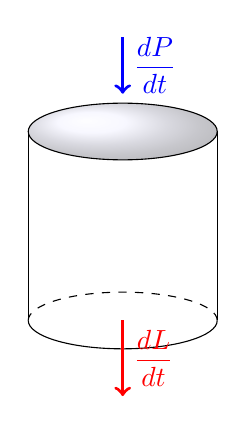
\begin{tikzpicture}[scale=1.2]

        % Draw cylinder (as a can)
        \shade[ball color=blue!10, opacity=0.4] (0,0) ellipse (1 and 0.3); % top ellipse
        \draw (0,0) ellipse (1 and 0.3);
        \draw (-1,0) -- (-1,-2);
        \draw (1,0) -- (1,-2);
        \draw (-1,-2) arc (180:360:1 and 0.3);
      
        % Hide back part of bottom ellipse
        \draw[dashed] (1,-2) arc (0:180:1 and 0.3);
      
        % Arrow pouring in (top)
        \draw[->, very thick, blue] (0,1) -- (0,0.4) node[midway,right] {$\dfrac{dP}{dt}$};
      
        % Arrow leaking out (bottom)
        \draw[->, very thick, red] (0,-2) -- (0,-2.8) node[midway,right] {$\dfrac{dL}{dt}$};
      
      \end{tikzpicture}
\end{center}

It's clear that the rate of change of total volume of water in the can is the differential equation $\dfrac{dV}{dt} = \dfrac{dP}{dt} - \dfrac{dL}{dt}$. However, what if I have two cans, with one leaking into the other? 

\begin{center}
    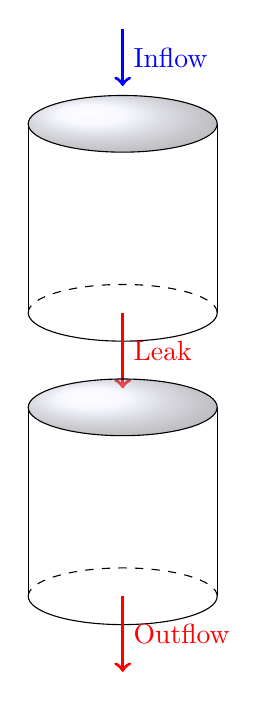
\begin{tikzpicture}[scale=1.2]

        % ---------- Top Cylinder ----------
        \coordinate (TopCylTop) at (0,0);
        \coordinate (TopCylBottom) at (0,-2);
        
        % top ellipse
        \shade[ball color=blue!10, opacity=0.4] (TopCylTop) ellipse (1 and 0.3);
        \draw (TopCylTop) ellipse (1 and 0.3);
        
        % sides
        \draw (-1,0) -- (-1,-2);
        \draw (1,0) -- (1,-2);
        
        % bottom ellipse
        \draw (-1,-2) arc (180:360:1 and 0.3);
        \draw[dashed] (1,-2) arc (0:180:1 and 0.3);
        
        % inflow arrow
        \draw[->, very thick, blue] (0,1) -- (0,0.4) node[midway,right] {Inflow};
        
        % leak arrow to bottom cylinder
        \coordinate (TopLeak) at (0,-2);
        \draw[->, very thick, red] (TopLeak) -- (0,-2.8) node[midway,right] {Leak};
        
        % ---------- Bottom Cylinder ----------
        \coordinate (BotCylTop) at (0,-3);
        \coordinate (BotCylBottom) at (0,-5);
        
        % top ellipse
        \shade[ball color=blue!10, opacity=0.4] (BotCylTop) ellipse (1 and 0.3);
        \draw (BotCylTop) ellipse (1 and 0.3);
        
        % sides
        \draw (-1,-3) -- (-1,-5);
        \draw (1,-3) -- (1,-5);
        
        % bottom ellipse
        \draw (-1,-5) arc (180:360:1 and 0.3);
        \draw[dashed] (1,-5) arc (0:180:1 and 0.3);
        
        % outflow arrow from bottom cylinder
        \draw[->, very thick, red] (0,-5) -- (0,-5.8) node[midway,right] {Outflow};
        
        \end{tikzpicture}
\end{center}

This would result in a \textbf{system of differential equations}, which ties together the linear algebra and the differential equations portion of this class.

\end{document}